% $Id$

In this chapter, we use the techinques developed in the previous chapters to
to search for gravitational waves from binary black hole MACHO inspiral in
data from the second LIGO science run. The goal of the search is to detect the
gravitational waves emitted by the late stages of inspiral. In the absence of
detection, however, we may place an \emph{upper limit} on the rate of
inspiraling BBHMACHOs which may be compared this to the predicted rate of $5
\times 10^{-2} \times 2^{\pm 1}$ discussed in chapter \ref{ch:macho}. In
section \ref{s:s2run} we describe the data sample used in the analysis.
Section \ref{s:s2tuning} describes how the parameters of the search listed in
the previous chapter were tuned on the playground data. Section
\ref{s:monte}.



Here we present the analysis of the
\emph{playground data}



\section{The Second LIGO Science Run}
\label{s:s2run}

All three LIGO detectors operated during the second LIGO science run, referred
to as S2, which spanned 59 days (1415 hours) from February 14 to April 14,
2003. While the detailed noise spectrum of a detector affects different
gravitational wave searches in different ways, we can summarize the
sensitivity of an detector for low-mass inspiral signals in terms of the
distance to which an {\em optimally oriented} binary system with component
masses of $1.4 M_\odot$ (and located at the detector's zenith, with its
orbital plane parallel to the plane defined by the detector arms) would yield
an amplitude signal-to-noise ratio (SNR) of 8 when extracted from the data
using optimal filtering. 

Although the detectors were manned by operators and scientists 24 hours per
day, the amount of science data with good performance and stable operating
conditions was limited by environmental factors (especially high ground motion
at LLO and strong winds at LHO), occasional equipment failures, and periodic
special investigations.  The total amount of science data obtained was 536
hours for L1, 1044 hours for H1, and 822 hours for H2.

The analysis described in this thesis uses data collected while the LLO
detector was operating at the same time as one or both of the LHO detectors.
Science data during which both H1 and H2 were operating but L1 was not,
amounting to 383 hours, was not used in this analysis because of
concerns about possible environmentally-induced correlations between the data
streams of these two co-located detectors; this data set, as well as data
collected while only one of the LIGO detectors was in science mode, will be
combined with data from the third LIGO science run in a future analysis.

\begin{figure}[H]
\begin{center}
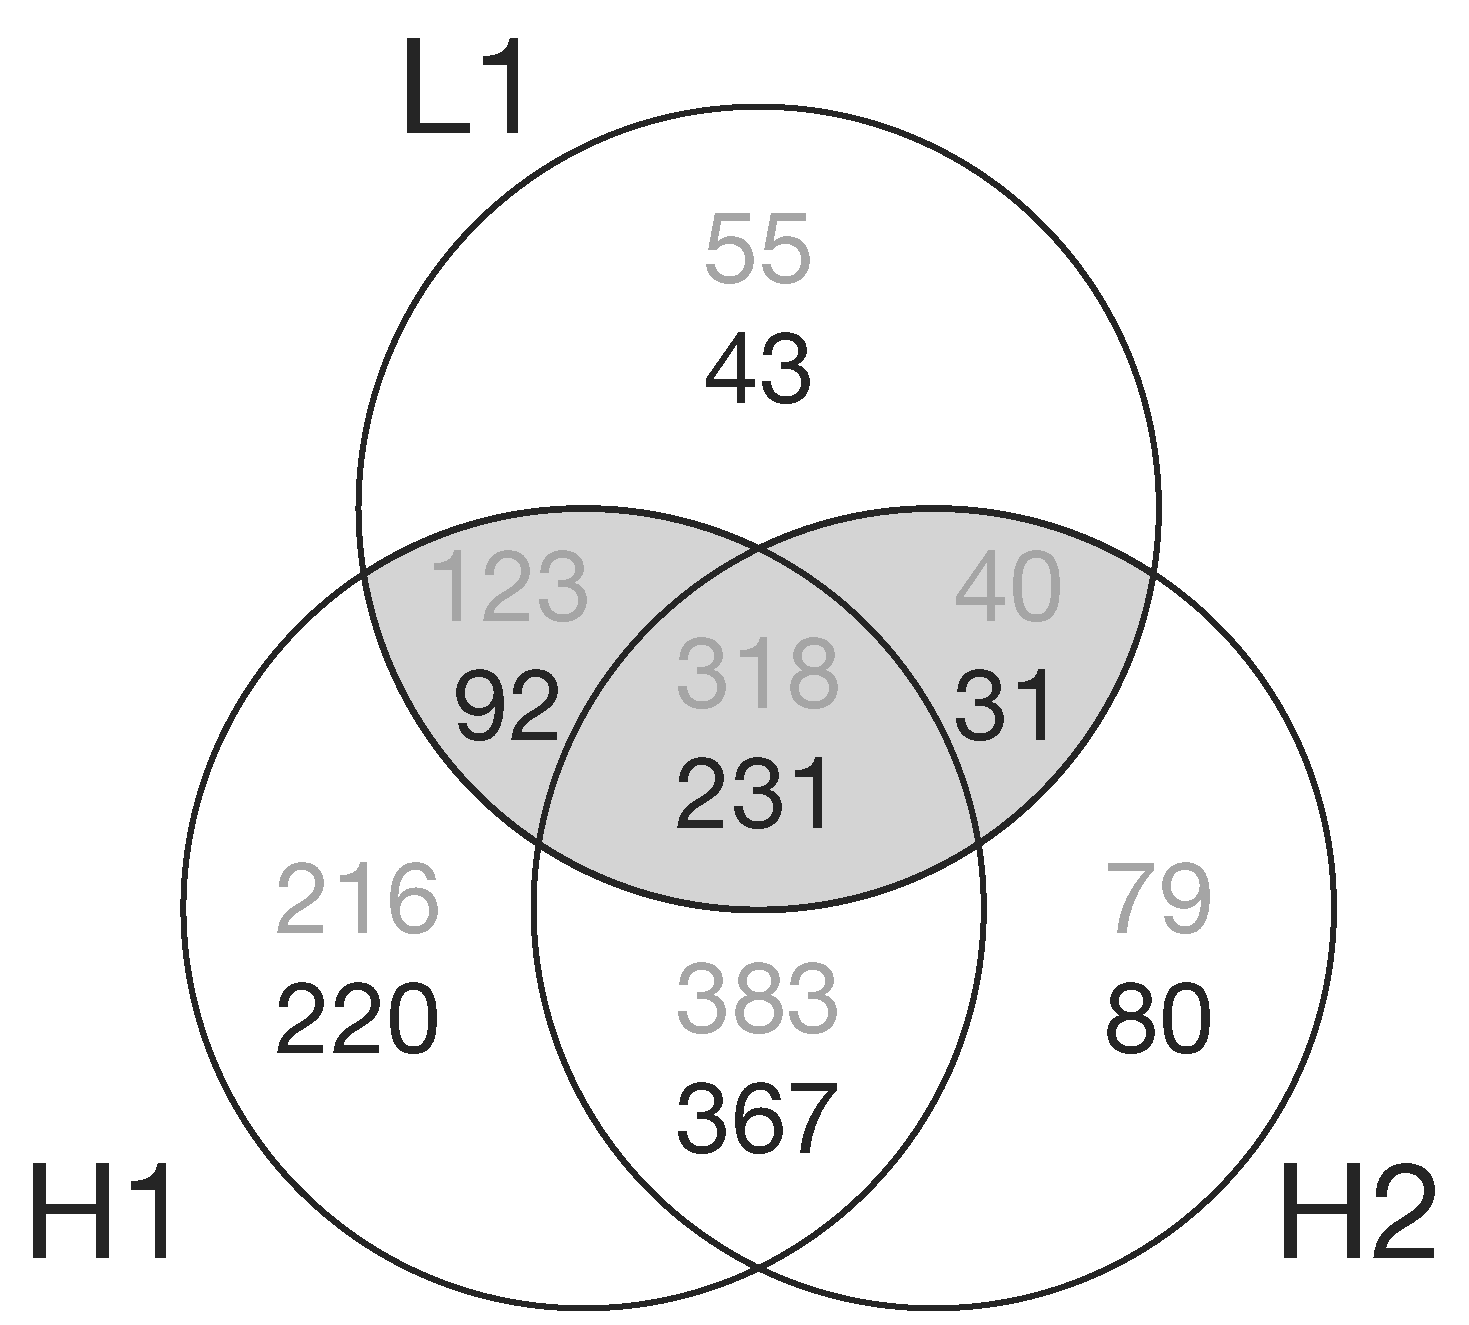
\includegraphics[width=\linewidth]{figures/result/s2_times}
\end{center}
\caption{\label{f:S2times}%
The number of hours that each detector combination was operational during the
S2 run.  The upper number gives the amount of time the specific instruments
were coincidentally operational.  The lower number gives the total
non-playground time which was searched for inspiral triggers.  The shaded
region corresponds to the data used in this search.}
\end{figure}


\section{Tuning the Analysis Pipeline}
\label{s:s2tuning}


\section{Injection Monte Carlos}
\label{s:monte}

\section{Accuracy of Parameter Measurement}
\label{ss:s2parameters}

\section{Search Efficiency}
\label{ss:s2efficiency}

\section{Background Estimation}
\label{s:s2background}

\section{Playground Upper Limit and Projection to Full Data Set}
\label{s:s2upperlimit}























\newpage

\begin{figure}[p]
\begin{center}
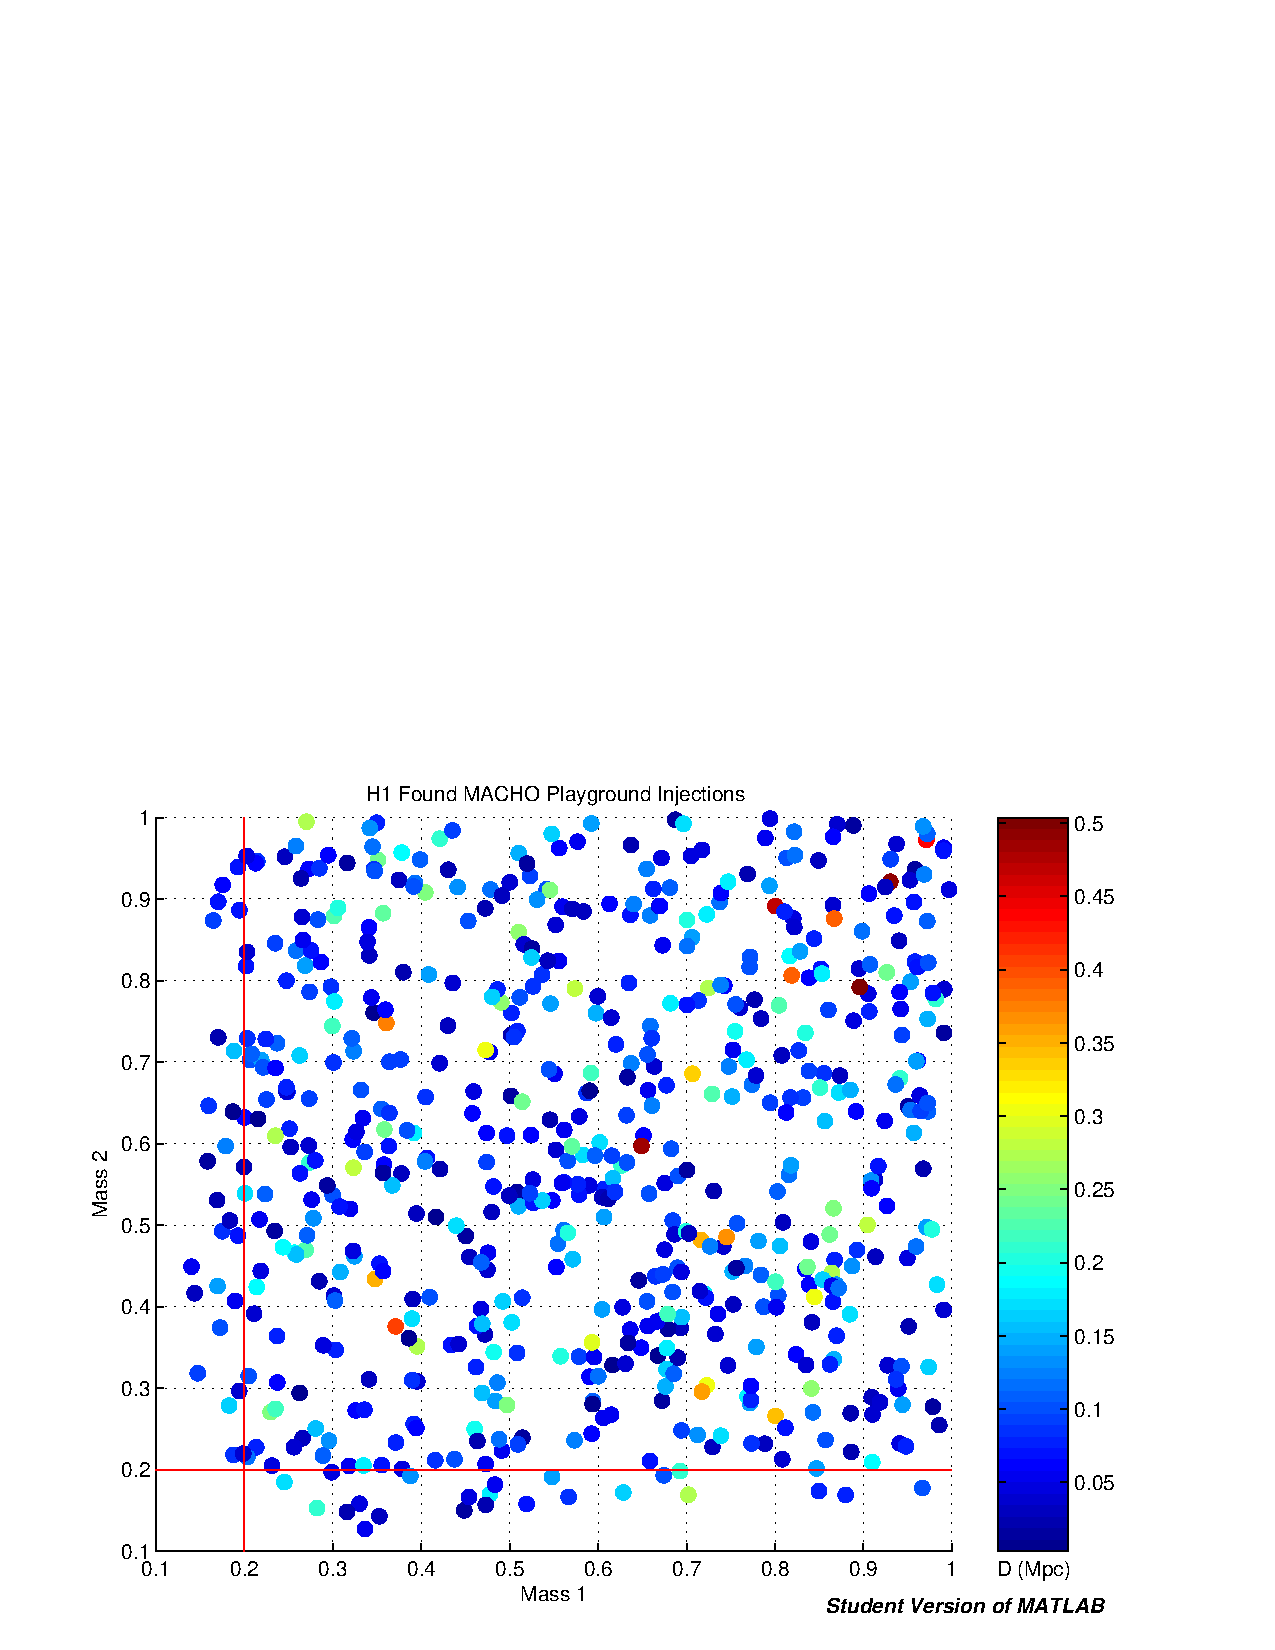
\includegraphics[width=\textwidth]{analysis/figures/m1m2_found}
\end{center}
\caption{\label{f:m1m2_found}%
Found injections.
}
\end{figure}

\begin{figure}[p]
\begin{center}
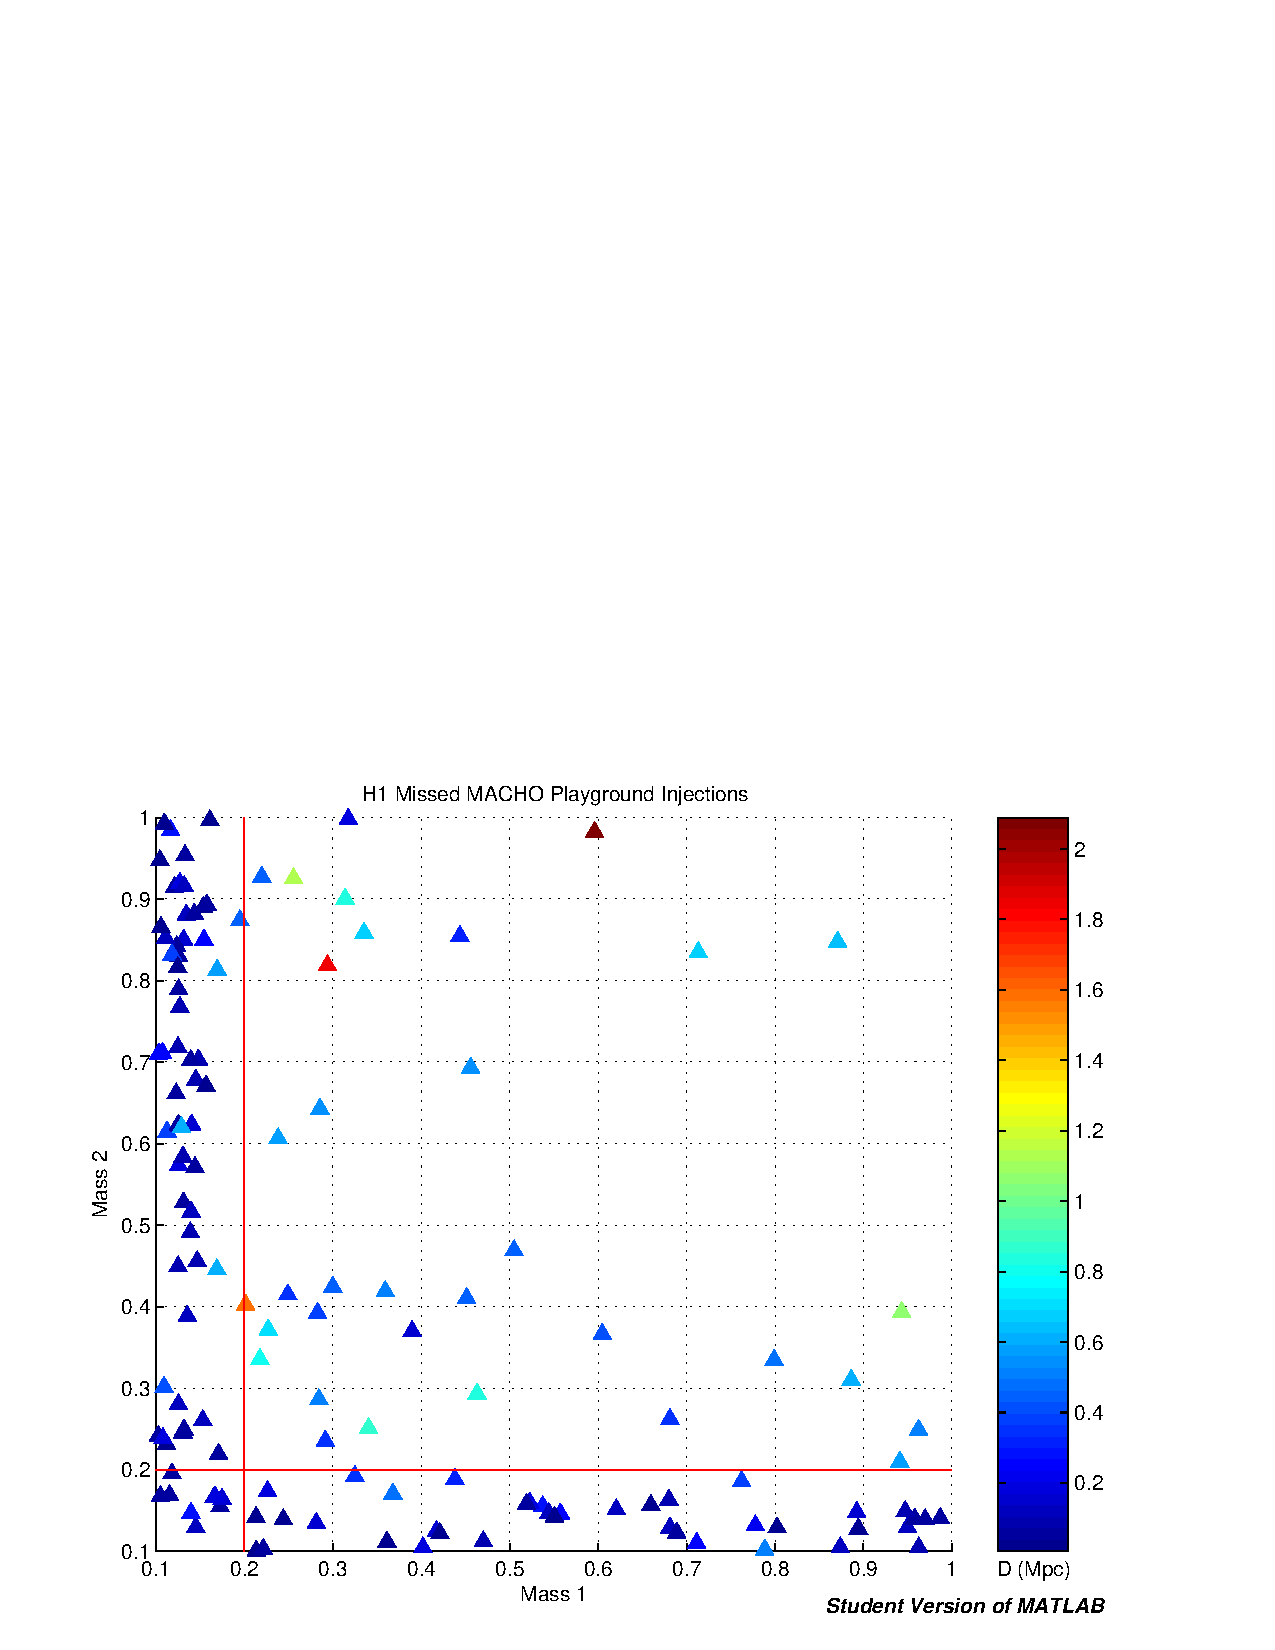
\includegraphics[width=\textwidth]{analysis/figures/m1m2_missed}
\end{center}
\caption{\label{f:m1m2_missed}%
Found injections.
}
\end{figure}


\begin{figure}[p]
\begin{center}
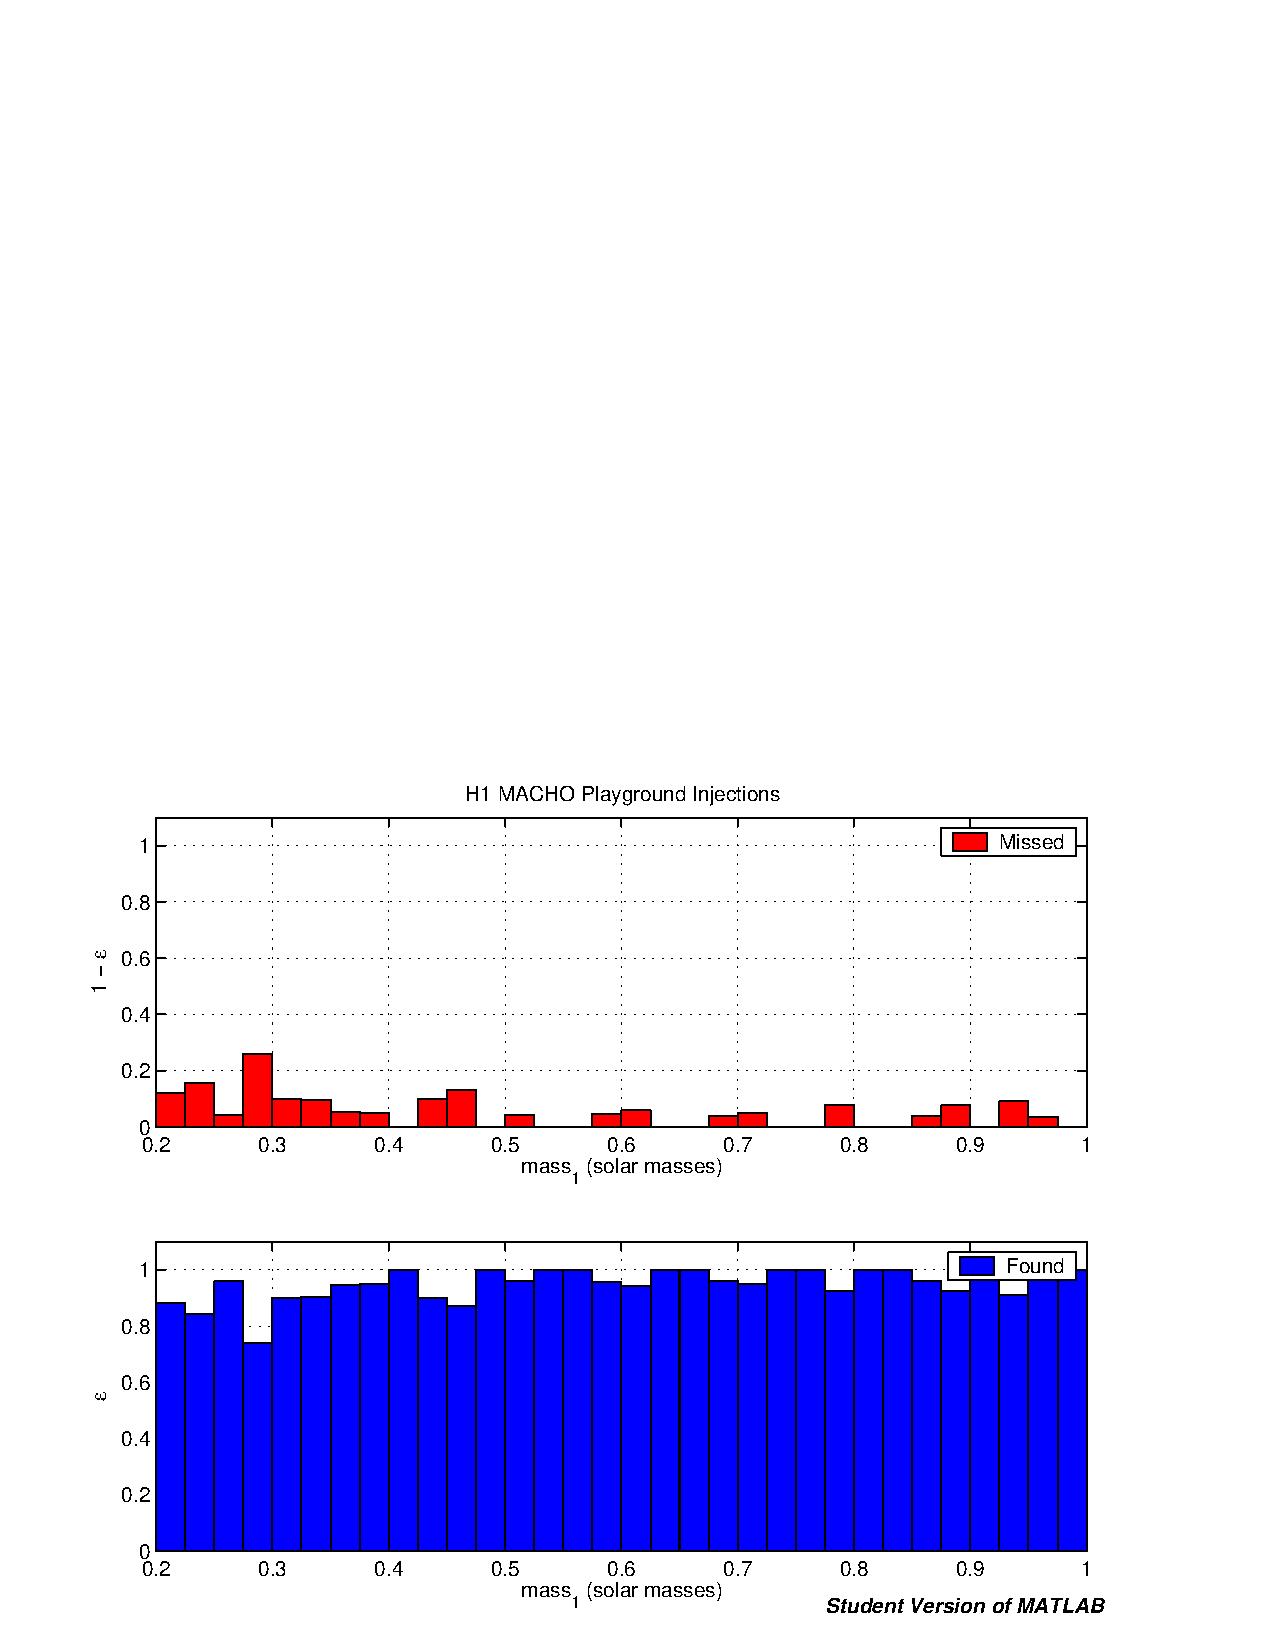
\includegraphics[width=\textwidth]{analysis/figures/msun_eff} \\
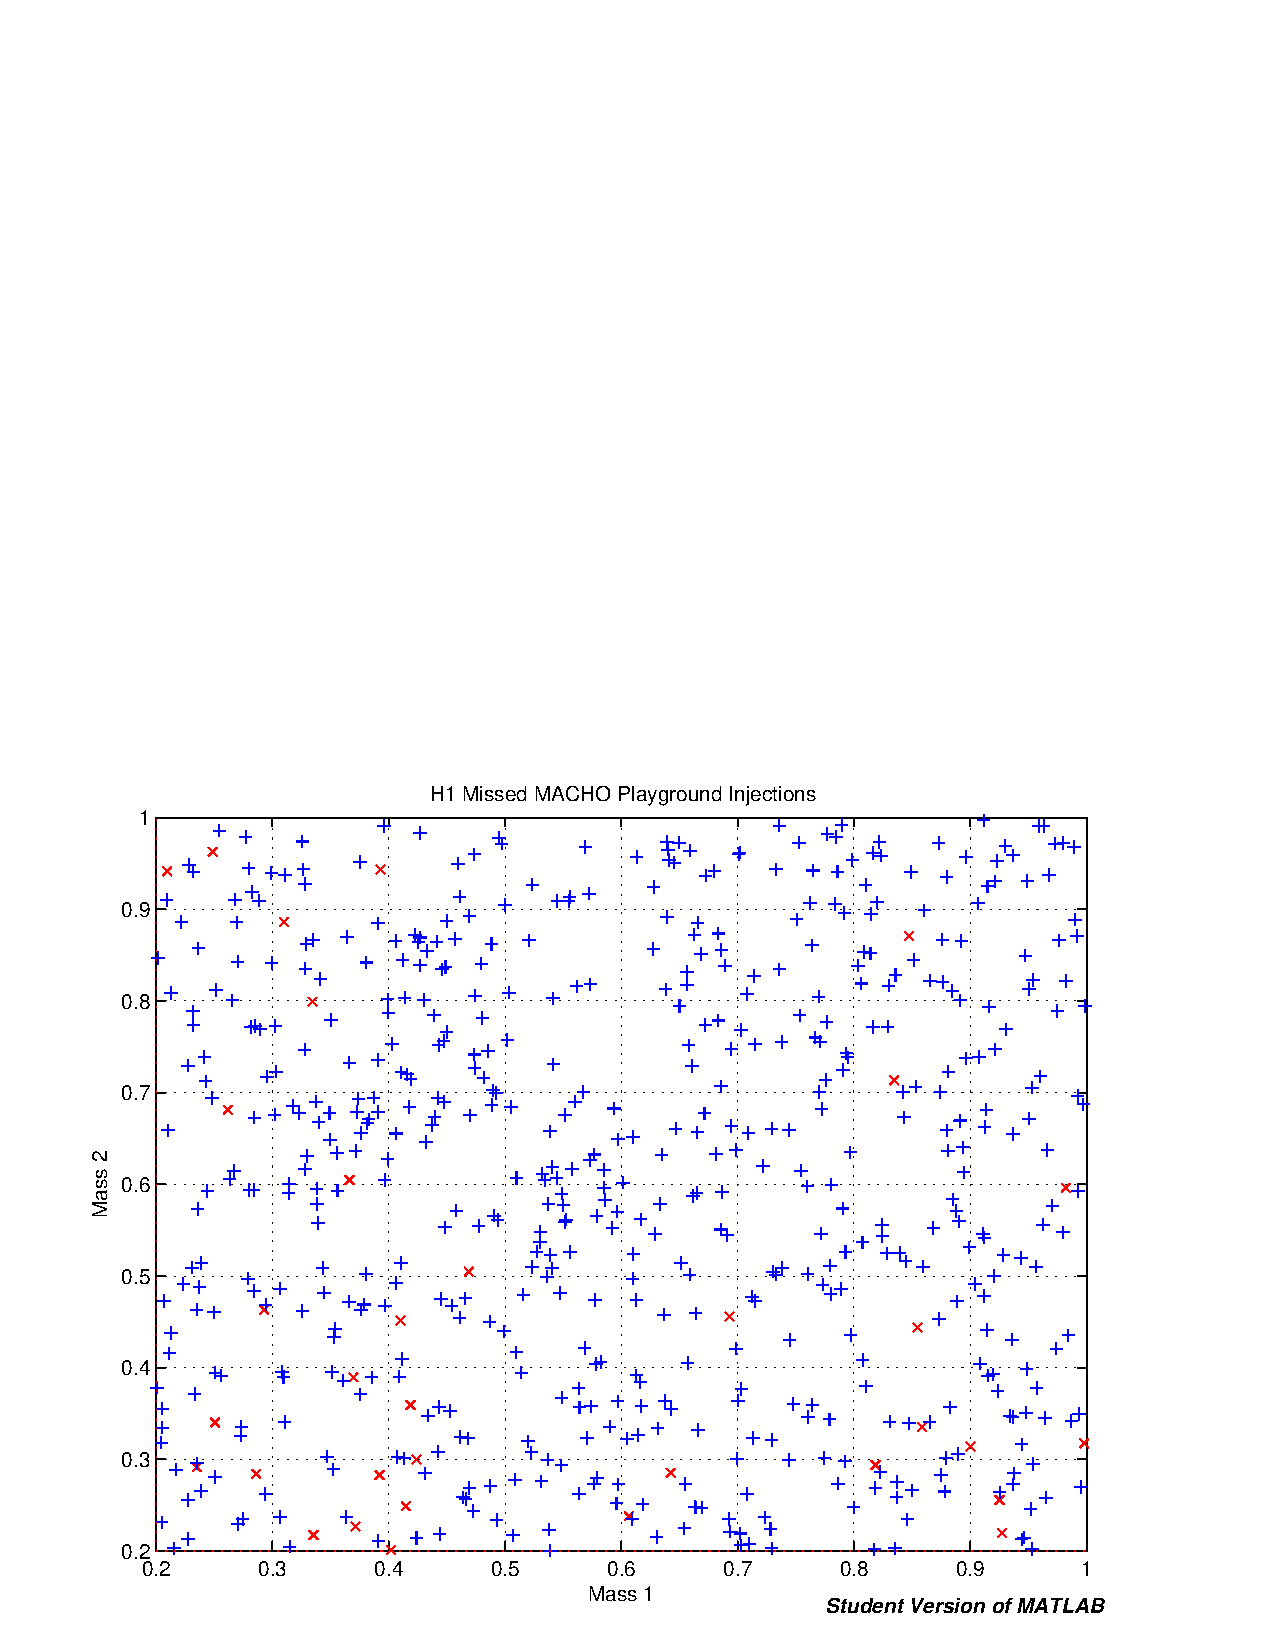
\includegraphics[width=\textwidth]{analysis/figures/m1m2_found_missed}
\end{center}
\caption{\label{f:msun_eff}%
Found injections.
}
\end{figure}

\begin{figure}[p]
\begin{center}
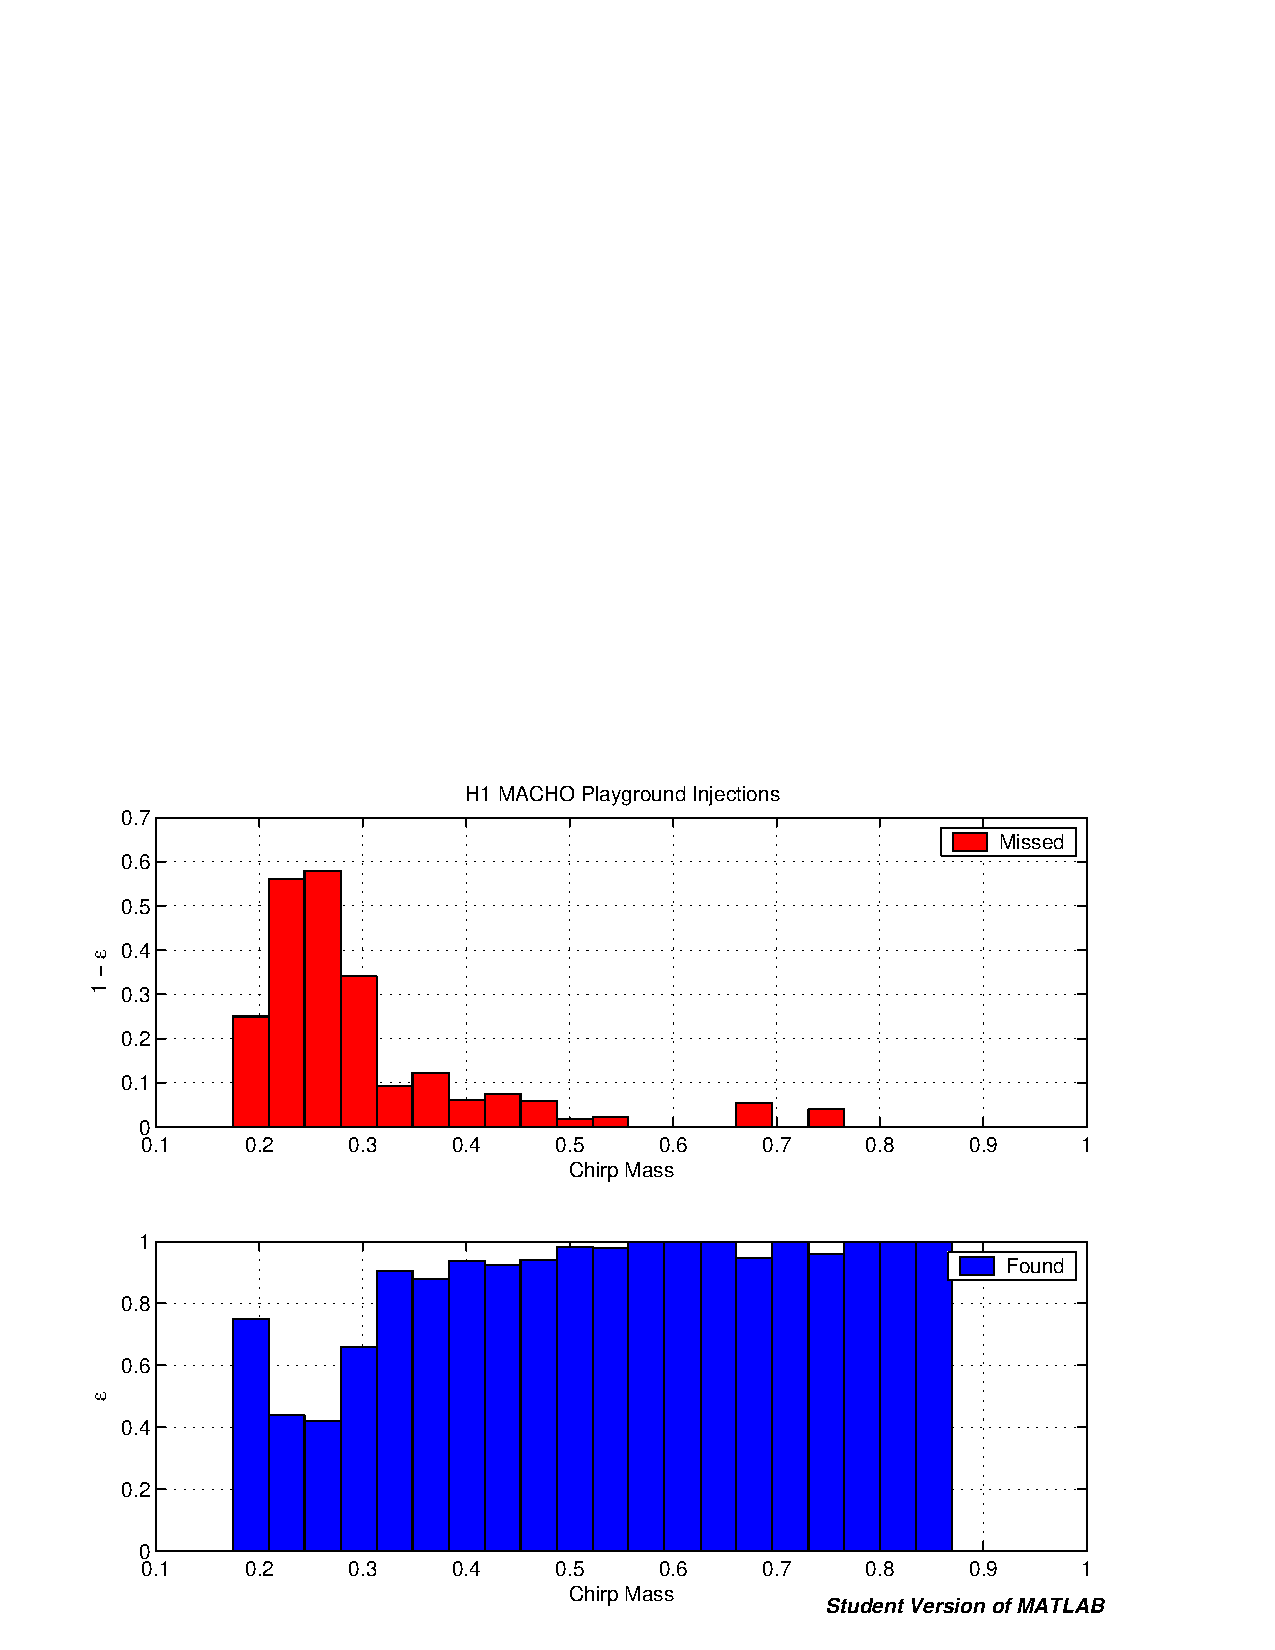
\includegraphics[width=\textwidth]{analysis/figures/mchirp_eff} \\
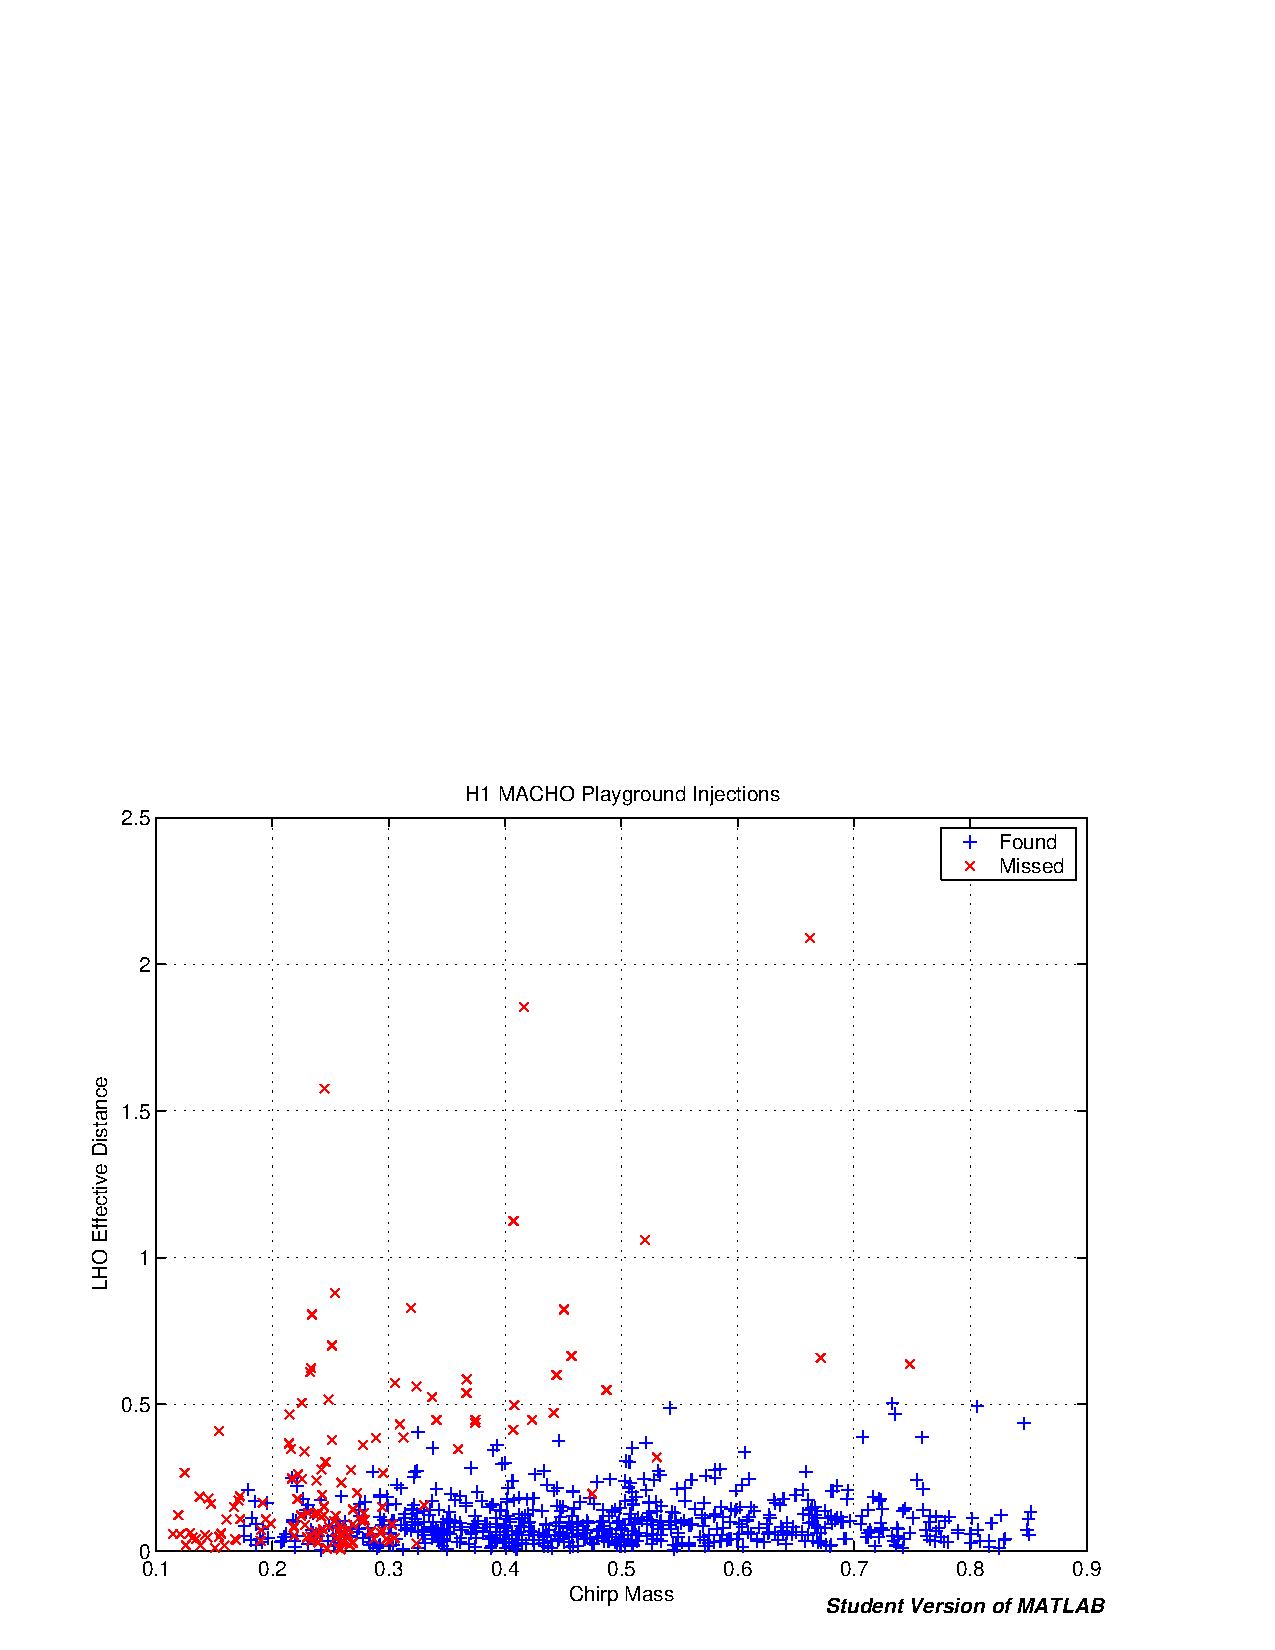
\includegraphics[width=\textwidth]{analysis/figures/mchirp_found_missed}
\end{center}
\caption{\label{f:mchirp_eff}%
Found injections.
}
\end{figure}

\begin{figure}[p]
\begin{center}
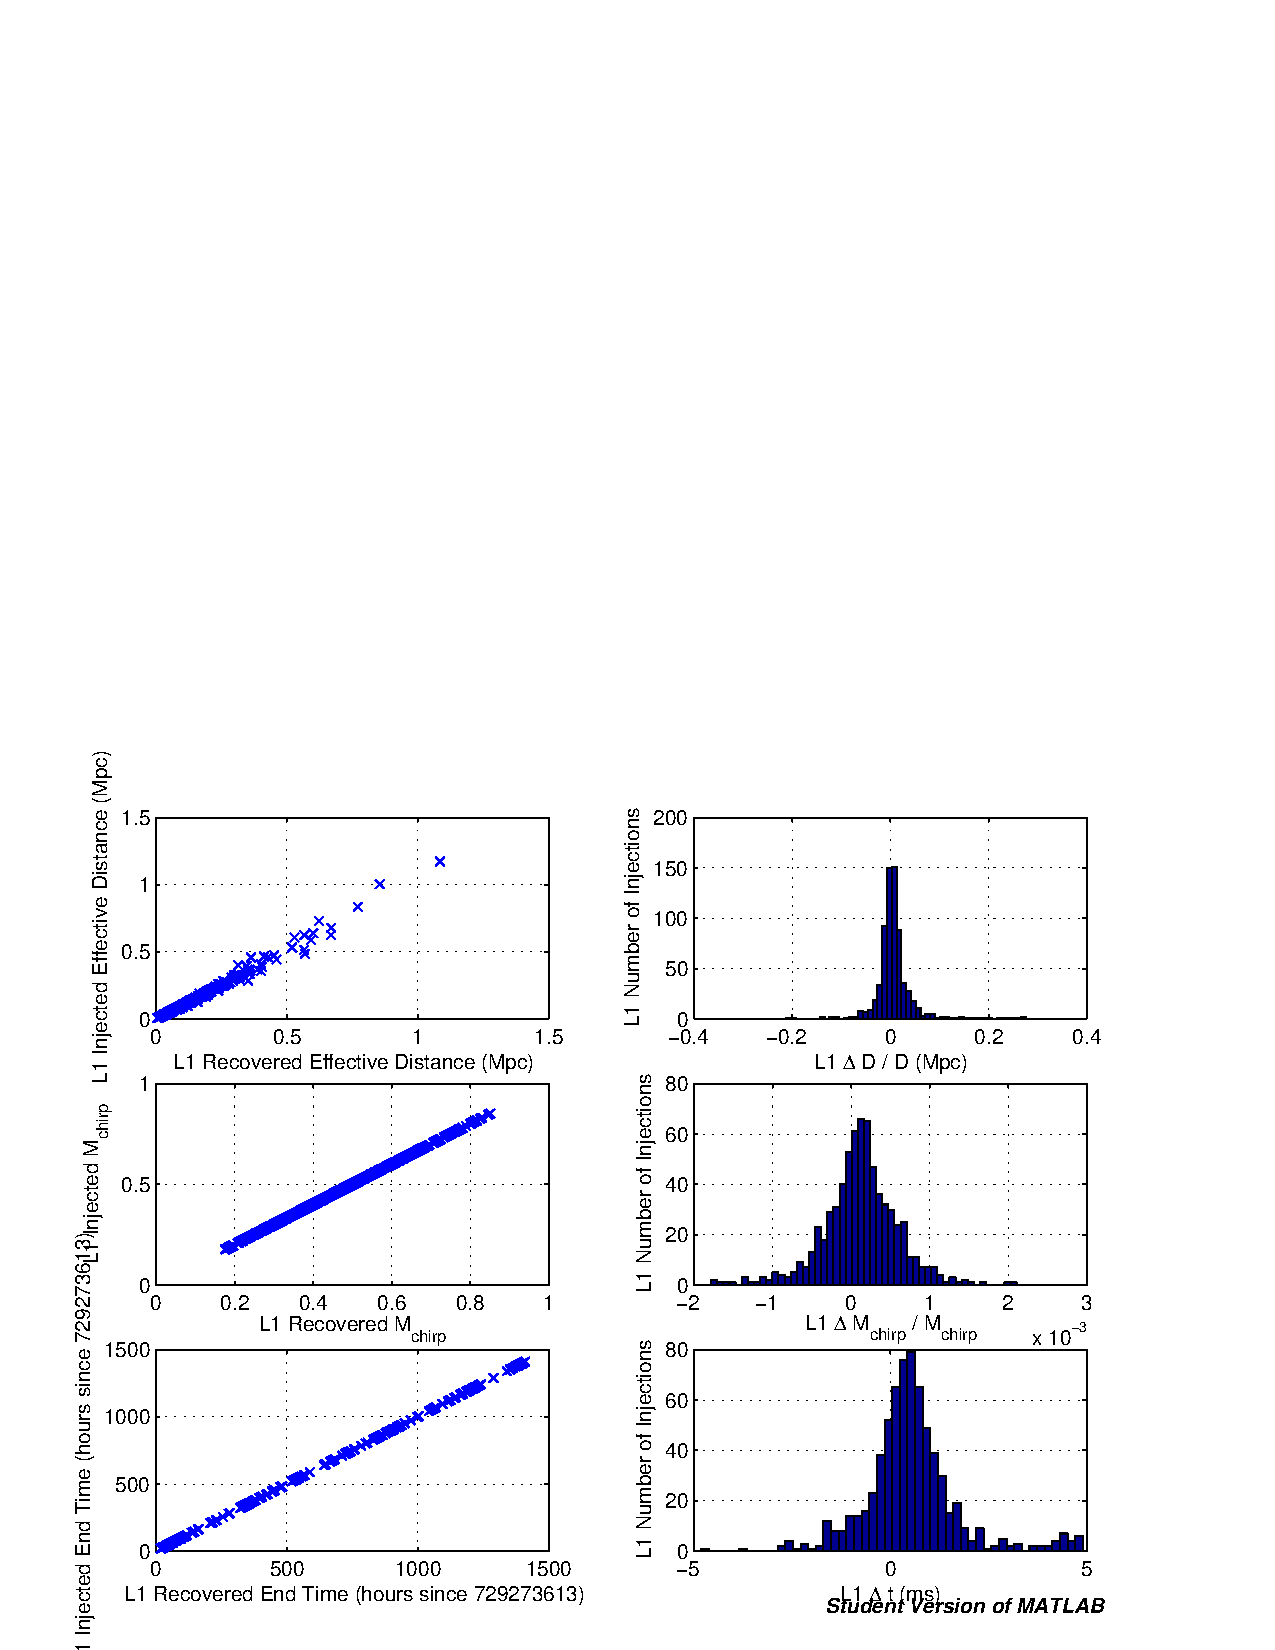
\includegraphics[width=\textwidth]{analysis/figures/l1_param_error}
\end{center}
\caption{\label{f:l1_param_error}%
Found injections.
}
\end{figure}

\begin{figure}[p]
\begin{center}
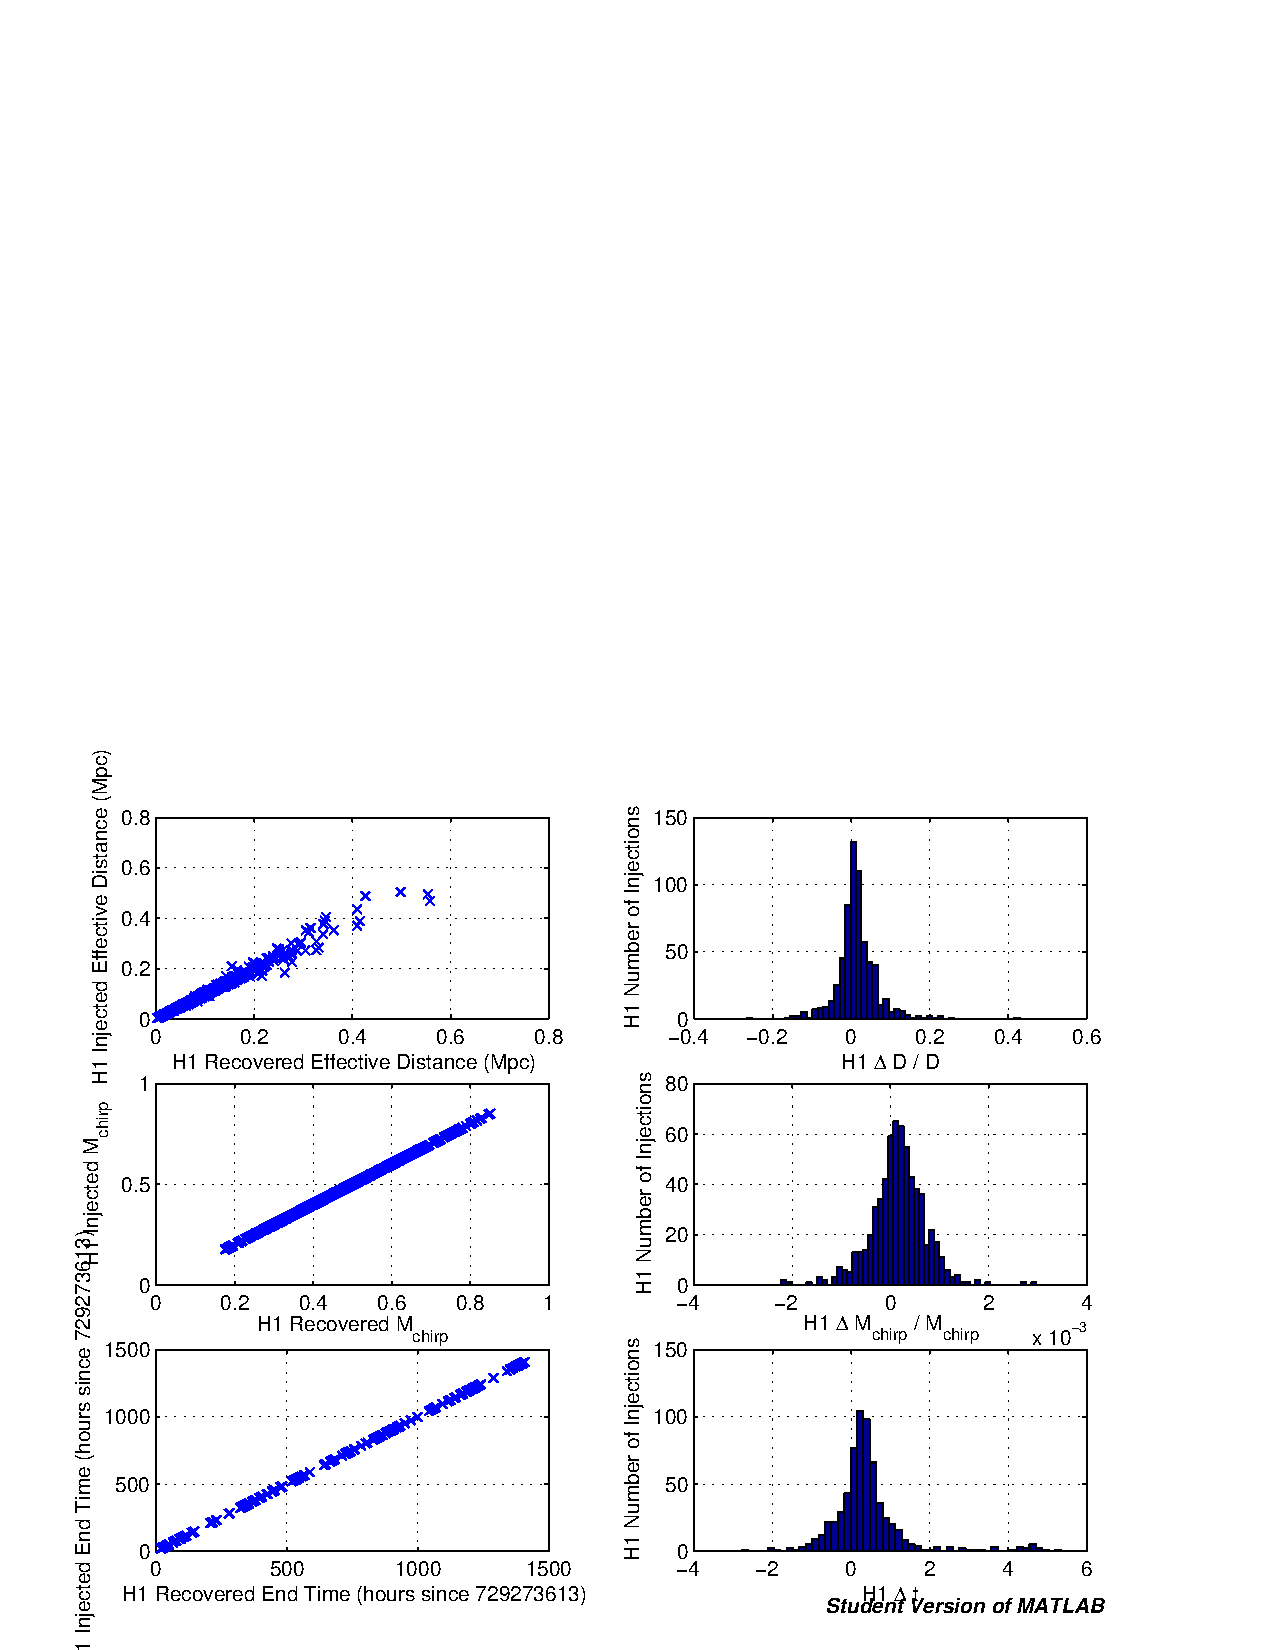
\includegraphics[width=\textwidth]{analysis/figures/h1_param_error}
\end{center}
\caption{\label{f:h1_param_error}%
Found injections.
}
\end{figure}

\begin{figure}[p]
\begin{center}
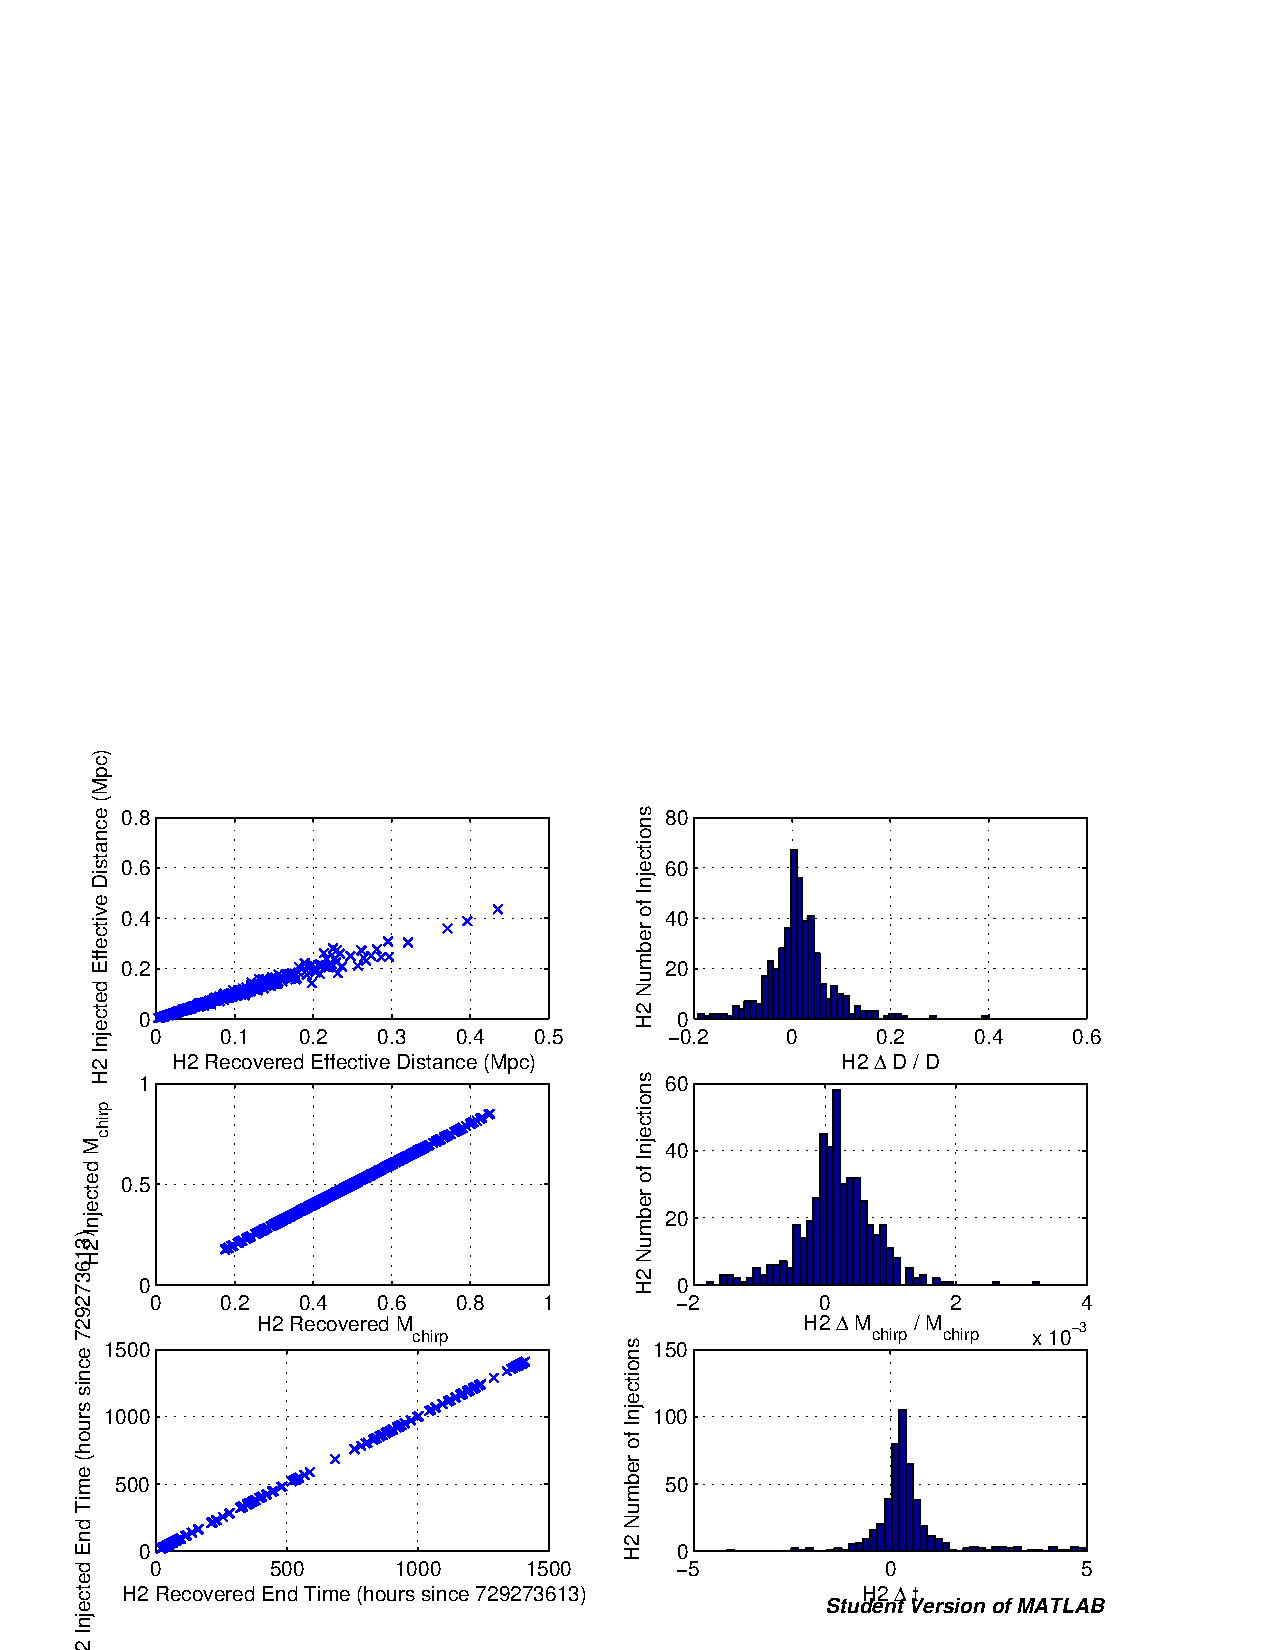
\includegraphics[width=\textwidth]{analysis/figures/h2_param_error}
\end{center}
\caption{\label{f:h2_param_error}%
Found injections.
}
\end{figure}

\begin{figure}[p]
\begin{center}
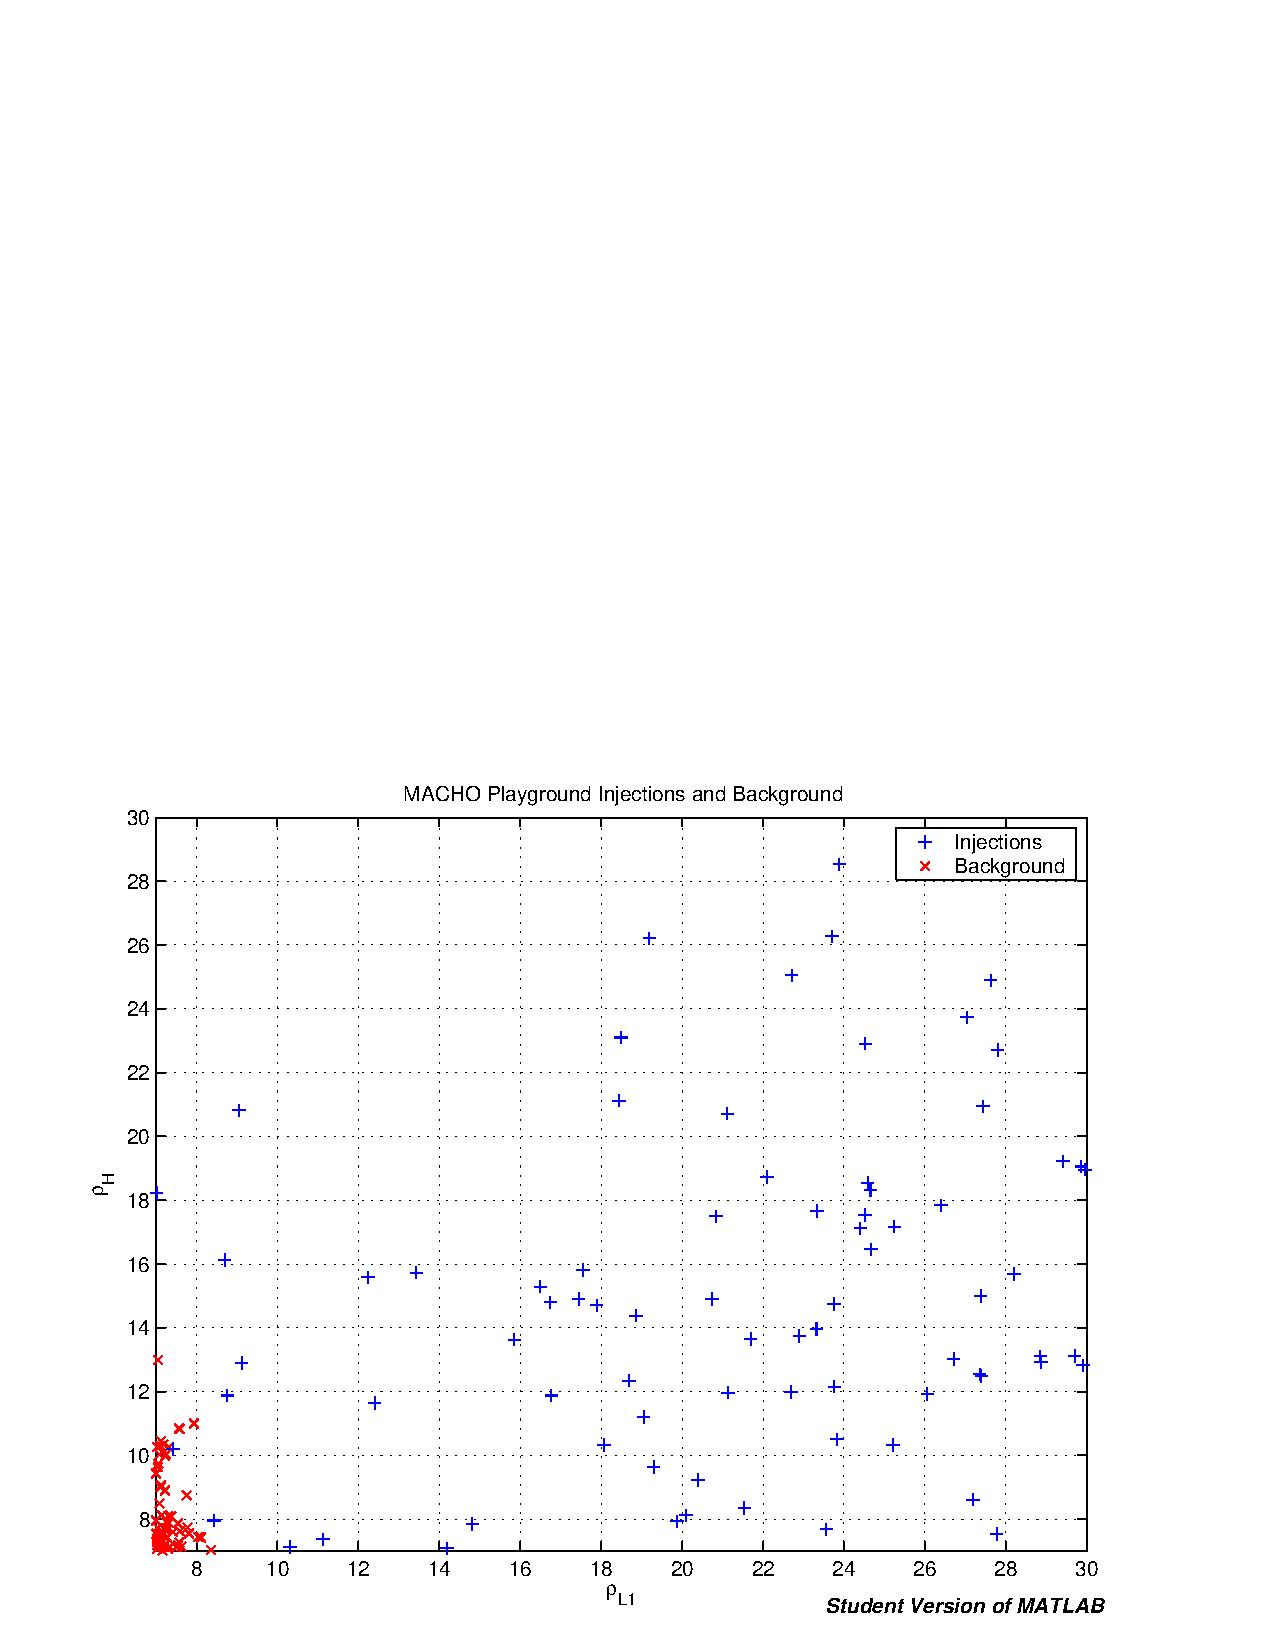
\includegraphics[width=\textwidth]{analysis/figures/inj_bkg_snr}
\end{center}
\caption{\label{f:inj_bkg_snr}%
Found injections.
}
\end{figure}

\begin{figure}[p]
\begin{center}
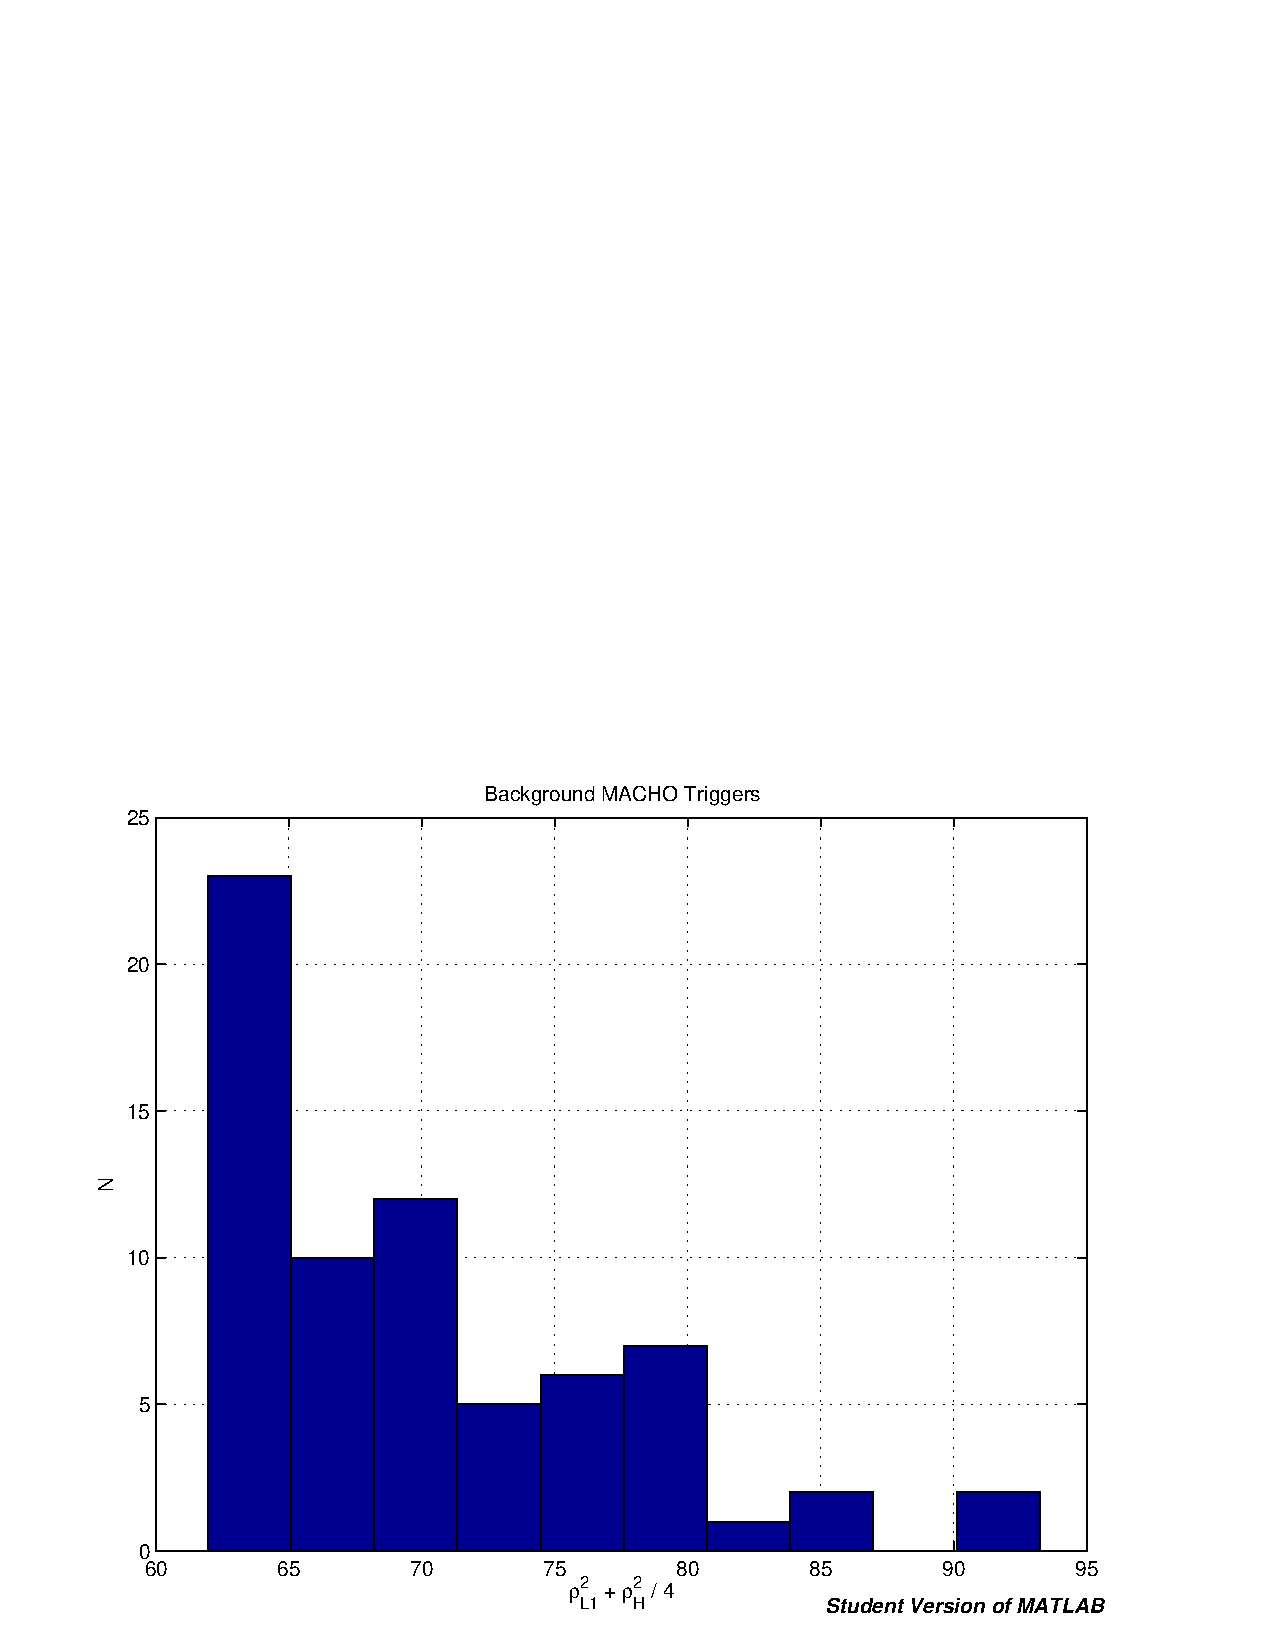
\includegraphics[width=\textwidth]{analysis/figures/bkg_hist}
\end{center}
\caption{\label{f:bkg_hist}%
Found injections.
}
\end{figure}

\begin{figure}[p]
\begin{center}
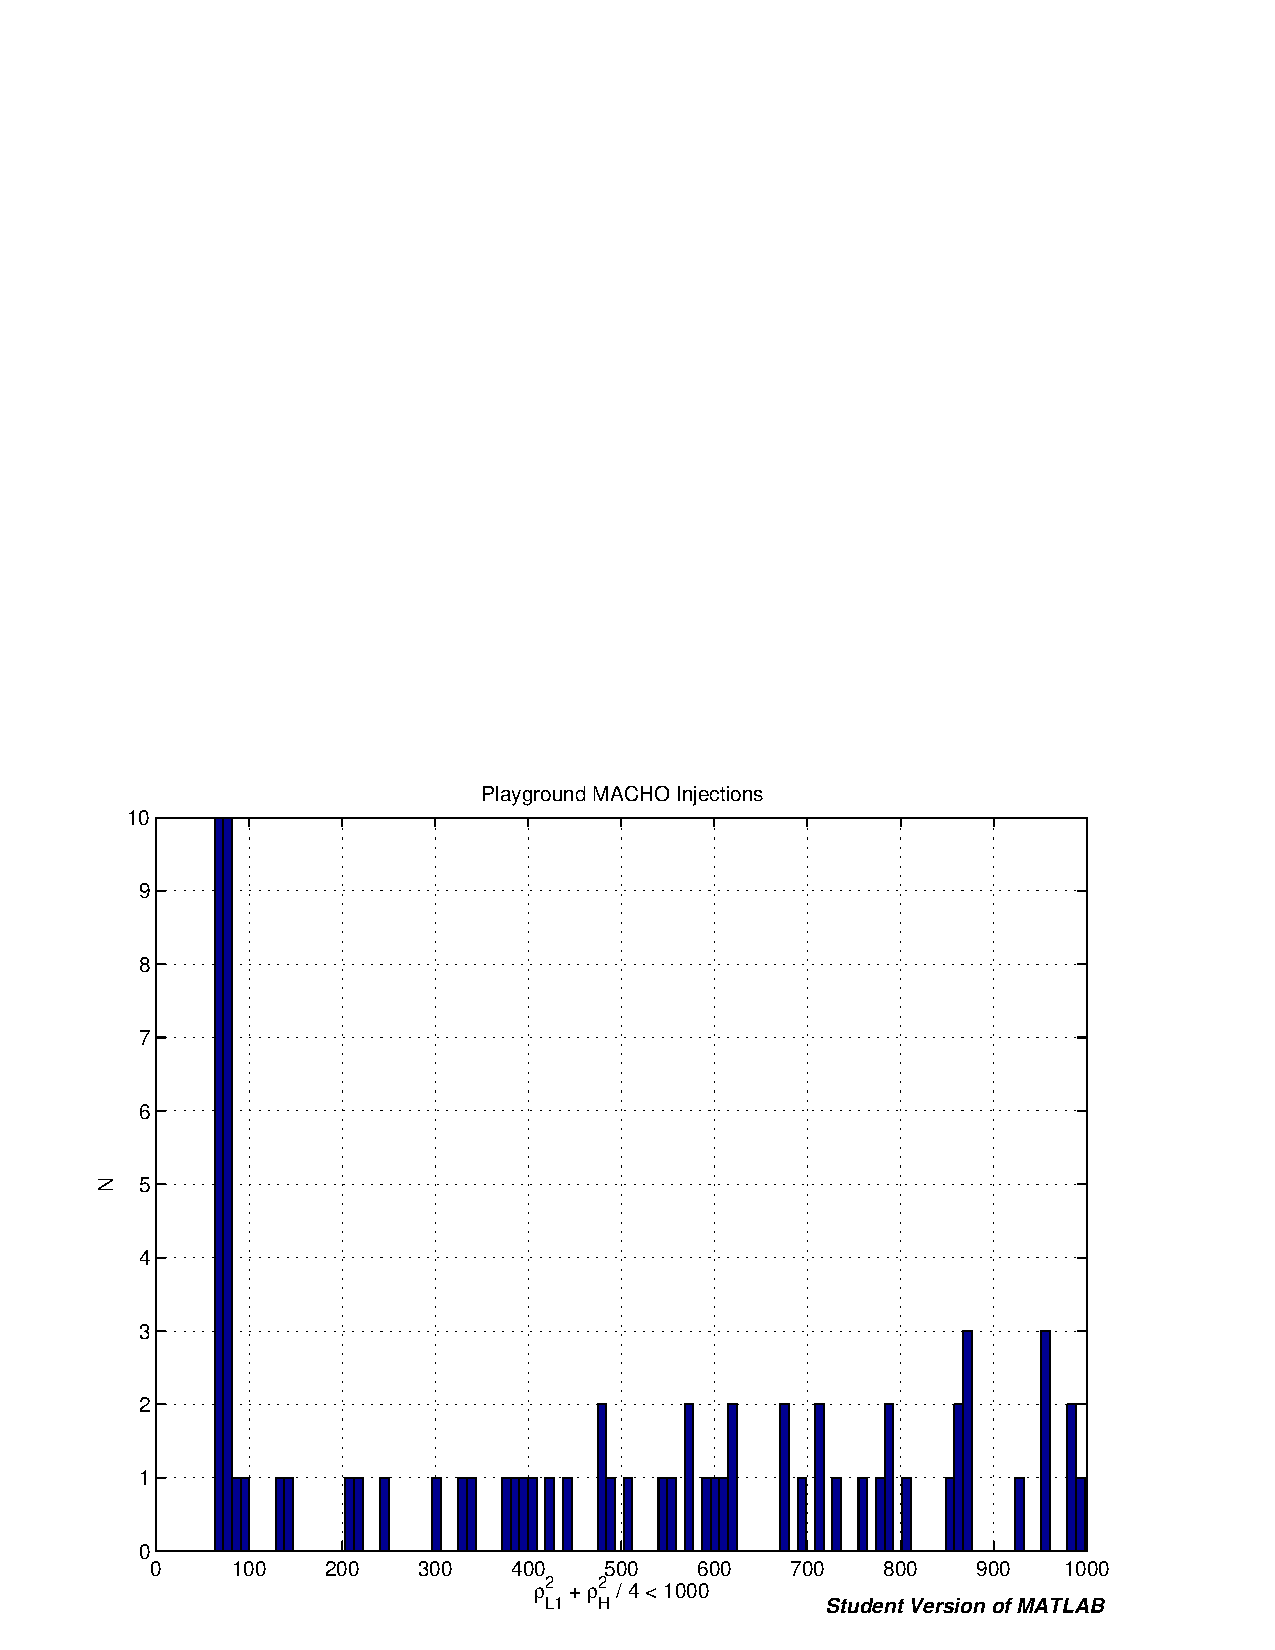
\includegraphics[width=\textwidth]{analysis/figures/inj_hist_lo}
\end{center}
\caption{\label{f:inj_hist_lo}%
Found injections.
}
\end{figure}

\begin{figure}[p]
\begin{center}
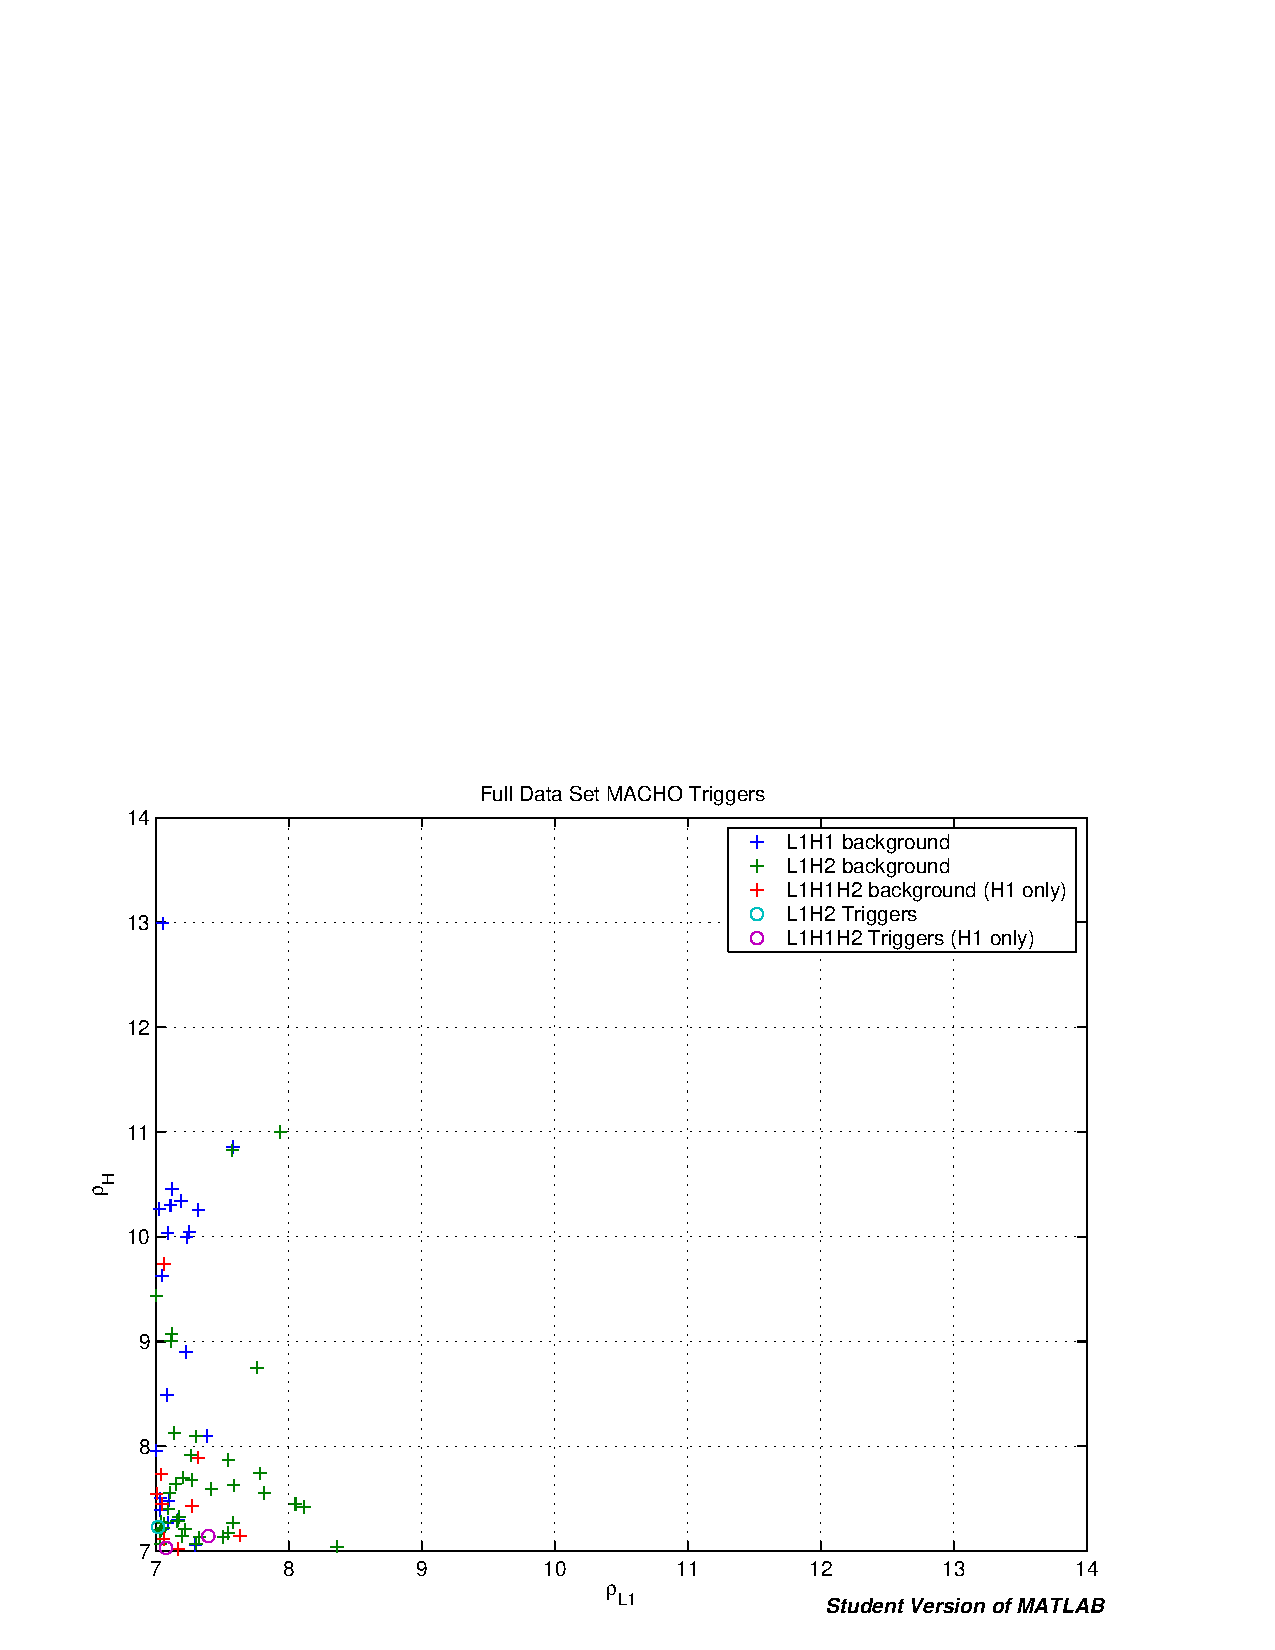
\includegraphics[width=\textwidth]{analysis/figures/bkg_fgd}\\
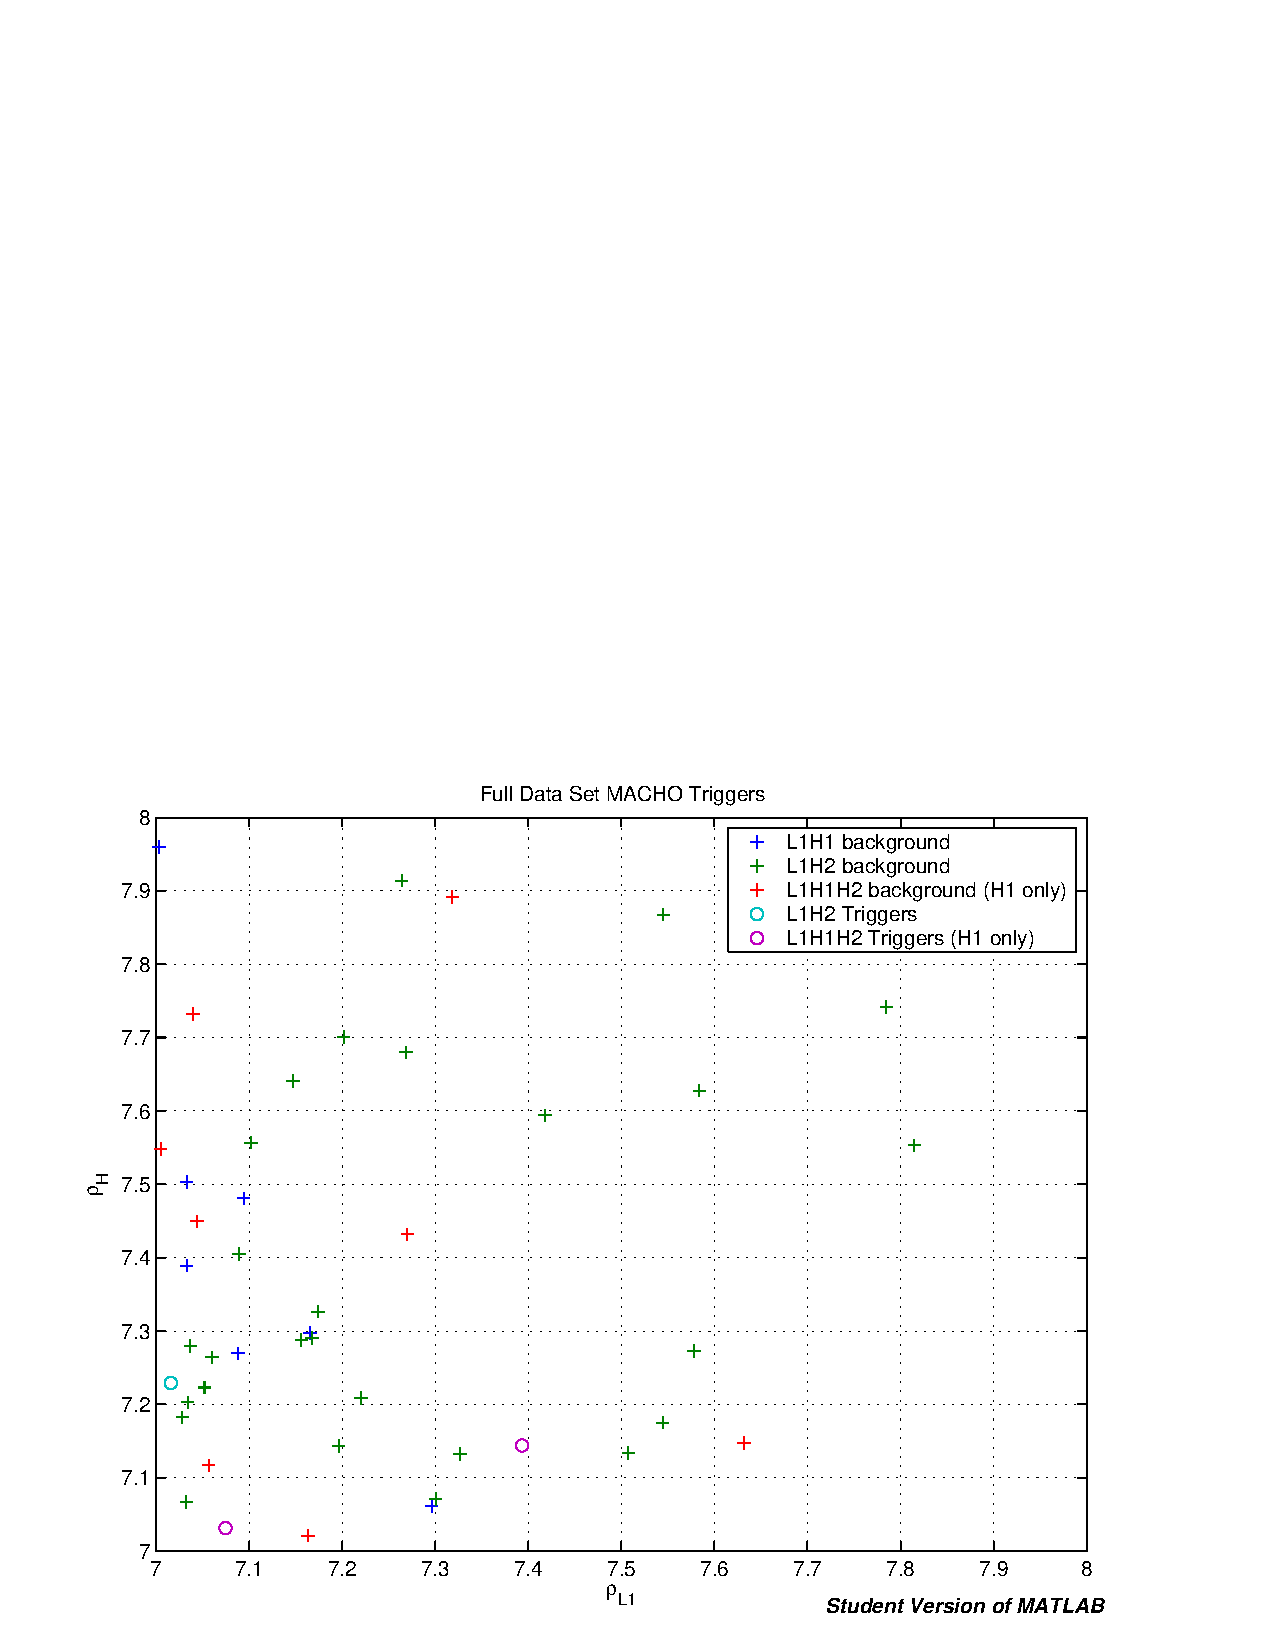
\includegraphics[width=\textwidth]{analysis/figures/bkg_fgd_zoom}
\end{center}
\caption{\label{f:bkg_found}%
Found injections.
}
\end{figure}
